\section{نمایش نقشه}
برای برنامه ریزی مسیر، ما به این احتیاج داریم که به یک شکلی محیط را در کامپیوتر نشان دهیم.
ما بین دو روش تکمیل کننده تقریب گسسته و پیوسته تفاوت قائل هستیم.
در تقریب گسسته ما نقشه را به قطعه های هم اندازه و یا اندازه های متفاوت
(مثل اتاق های یک ساختمان) تقسیم می کنیم. نقشه های دومی به نقشه های توپولوژیکال معروف هستند.
نقشه های گسسته را میتوان به راحتی به صورت گراف نمایش داد.
 در این حالت هر قطعه نقشه به عنوان راس های گراف در نظر گرفته می شوند
که به وسیله ی یال ها به هم اتصال پیدا می کنند اگر ربات بتواند از راسی به راس دیگر راه پیدا کند.
برای مثال نقشه ی جاده ها یک نقشه ی توپولوژیکال است که نقاط اتصال راس ها و جاده ها یال های هستند که با طولشان برچسب گذاری می شوند.
به صورت محاسباتی یک گراف می تواند  به صورت لیست یا ماتریس همسایگی یا وقوع
\lr{(adjacency or incidence list/matrix)}
ذخیره شود. در تقریب پیوسته داخلی (موانع) و خارجی مرز ها
که معمولا به شکل چند ضلعی نمایش داده می شود، مشخص می شود
که مسیر ها به صورت دنباله از اعداد حقیقی نمایش ک گذاری می شوند. 
با وجود برتری حافظه روش پیوسته، نقشه های پیوسته بیشتر در رباتیکز استفاده می شوند.
 
\par

برای نشان دادن موانع، یکی از نقشه های کارآمد نقشه شبکه ایی تصرف
\lr{(occupancy grid map)}
است. 
در نقشه شبکه ایی، محیط به مربع های با وضوح دلخواه تقسیم می شوند که روی آن موانع نشانه گذاری می شوند. 
در شبکه های تصرفی احتمالی در هر مربع درمورد احتمال حضور یک مانع بحث می شود. این موضوع زمانی 
که سنسور های ربات قطعیت ندارند اهمیت دارد. نقطه ضعف این روش مصرف شدن زیاد حافظه و 
همانطور زمان محاسباتی برای پیمایش ساختمان داده ها با راس های زیاد است. راه حل این مسئله استفاده 
از 
\lr{\textbf{k-d Tree}}
برای نمایش نقشه های شبکه ایی است. یک
\lr{k-d Tree}
 به صورت بازگشتی محیط را به
\lr{k}
 قطعه تقسیم میکند 
 برای مثال اگر
$k = 4$
باشد یکه ناحیه به چهار قسمت تقسیم می شود و 
هرکدوم از این بخش ها نیز خود به چهار بخش تقسیم می شوند تا به وضوح مورد نظر برسیم. در 
شکل
\ref{fig:quad-tree}
یک
\lr{quad-tree}
نشان داده شده است. همانطور که مشاهده می کنید در این درخت دیگر 
لازم نیست برای هر مربع یک برگ صرف کنیم و تعداد برگ های ما کمتر از تعداد مربع های شبکه است.
یک راه حل ایده آل وجود ندارد و برای هر کاربرد ممکن است راه حل های متفاوت نیاز باشد
که می توانند ترکیبی از همه آن ها باشند.
 



\begin{figure}[H]
  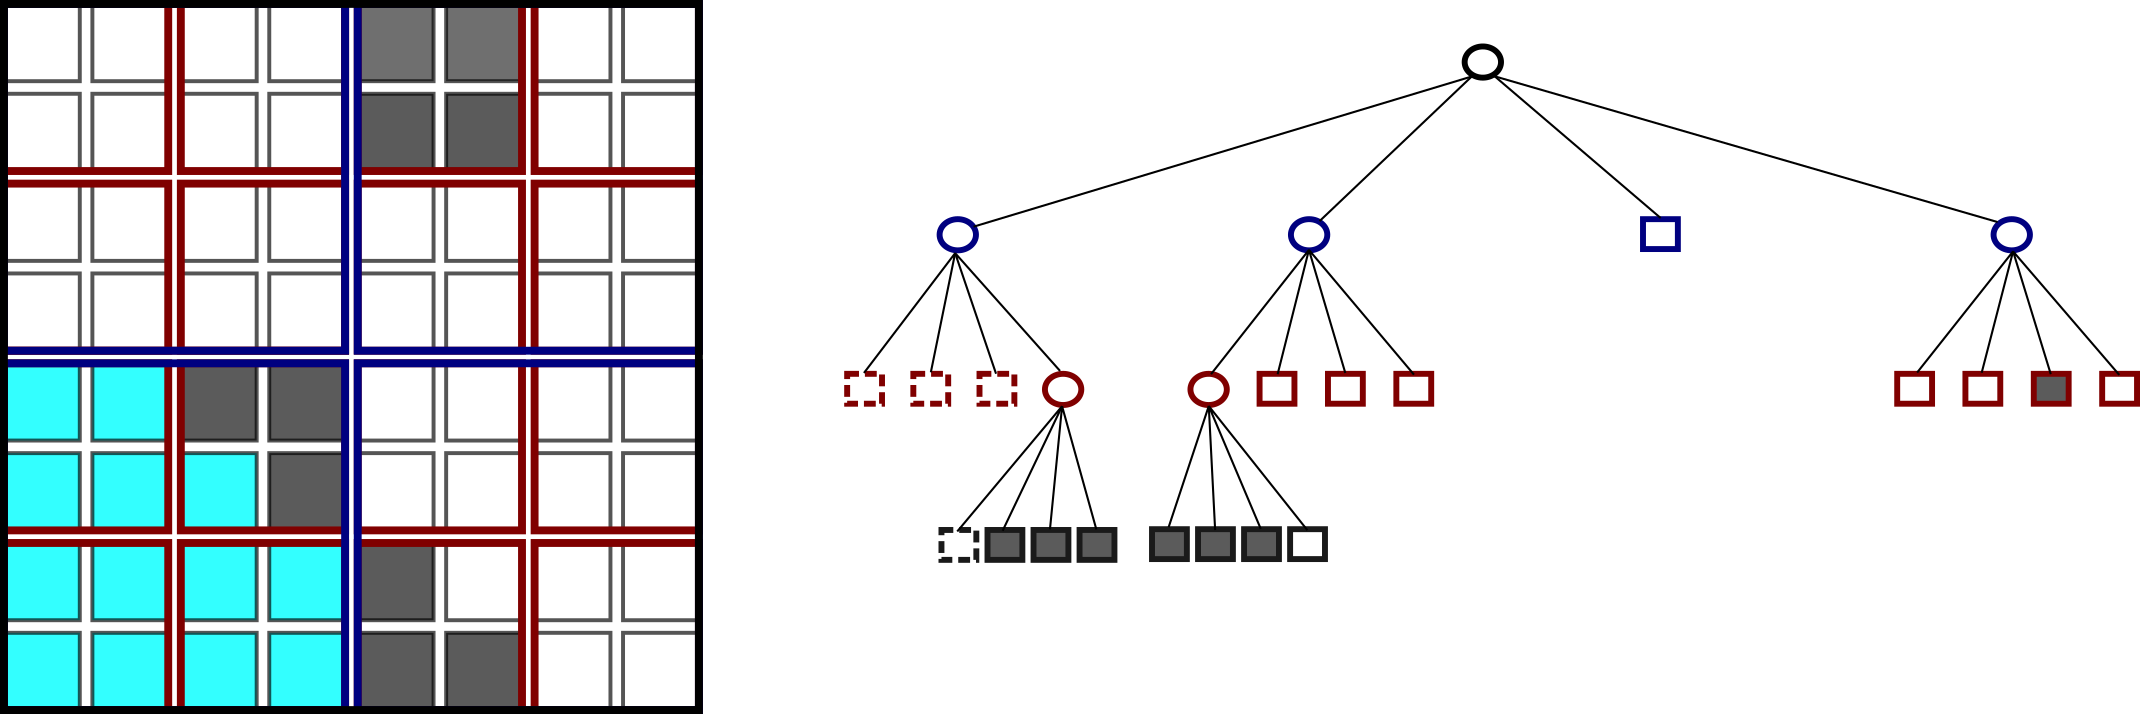
\includegraphics[width = \textwidth]{images/quad_tree.png}
  \caption{\lr{Quad Tree}}
  \label{fig:quad-tree}
\end{figure}
